\documentclass[aspectratio=169,10pt,xcolor=pdflatex,dvipsnames,table]{beamer}
\usepackage{newcent}
\usepackage[utf8]{inputenc}
\usepackage[czech]{babel}
\usepackage{hyperref}
\usepackage{amsthm}
\usepackage{amssymb}
\usepackage{amsmath}
\usepackage{array}
\usepackage{stmaryrd}
\usepackage{graphicx}
\usepackage{tabularx}
\usepackage{listings}
\usepackage{fancyvrb}
\usepackage{minted}
\usepackage{multicol}
%\usepackage{packages/beamerthemeFIT}

\makeatletter
  \def\beamer@calltheme#1#2#3{%
    \def\beamer@themelist{#2}
    \@for\beamer@themename:=\beamer@themelist\do
    {\usepackage[{#1}]{\beamer@themelocation/#3\beamer@themename}}}

  \def\usefolder#1{
    \def\beamer@themelocation{#1}
  }
  \def\beamer@themelocation{}

\usefolder{packages}
\usetheme{FIT}



\title[OpenGL]{PGR - Vertex Shader, Transformation}

\author[]{Tomáš Milet}

\institute[]{Brno University of Technology, Faculty of Information Technology\\
Bo\v{z}et\v{e}chova 1/2. 612 66 Brno - Kr\'alovo Pole\\
imilet@fit.vutbr.cz}

\date{\today}

\begin{document}

\frame[plain]{\titlepage}

% [normalized] vector
\newcommand{\V}[1]{\ensuremath{\mathbf{#1}}}
\newcommand{\NV}[1]{\ensuremath{\mathbf{\hat{#1}}}}

\begin{frame}
\frametitle{Matice a prostory}
	\begin{itemize}
		\item Model je namodelovaný v tzn. model space prostoru
    \item Vrcholy modelu se po vynásobení modelovou maticí přesunou do world space prostoru - prostoru scény
    \item Celá scéna se poté transformuje pomocí view matice tak, aby to simulovalo pohled z kamery
    \item Následuje projekce do clip space pomocí projekční matice
    \item Výstup vertex shaderu by měl být v clip space
	\end{itemize}
  \begin{figure}[h]
    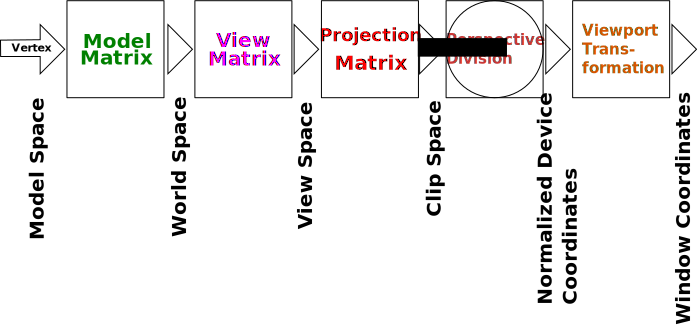
\includegraphics[width=10cm,keepaspectratio]{pics/linear/space.pdf}
  \end{figure}
\end{frame}


\begin{frame}
  \frametitle{Opakování Lingebry}
  Vektorový prostor
  \pause
  \begin{align*}
    \text{Vektory }\V{v}&(V,+,-) &
    \text{Skaláry }a&(S,+,-,*,{}^{-1})\\
    a(b\V{v}) &= (ab)\V{v} & 1\V{v} &= \V{v} \\
    a(\V{u}+\V{v}) &= a\V{u} + a\V{v} & (a+b)\V{v} &= a\V{v} + b\V{v}
  \end{align*}
  \pause
  Lineární kombinace
  \pause
  \begin{equation*}
    \V{v} = a_1\V{v}_1 + a_2\V{v}_2 + \dotsb + a_n\V{v}_n
  \end{equation*}
  \pause
  \begin{itemize}
    \item Lineární (ne)závislost
    \item Dimenze
    \item Báze
  \end{itemize}
\end{frame}

\begin{frame}
  \frametitle{Lineární transformace}
  $f$ zachovává lineární kombinaci :
  \begin{equation*}
    f(a_1\V{v}_1 + \dotsb + a_n\V{v}_n) = a_1f(\V{v}_1) + \dotsb + a_nf(\V{v}_n)
  \end{equation*}
  \pause
  Transformujeme $\V{v} = (x,y,z)^T$
  \begin{align*}
    \V{v} &= x\NV{x} + y\NV{y} + z\NV{z} & \NV{x} = (1,0,0)^T, \dotsc \\
    f(\V{v}) &= xf(\NV{x}) + yf(\NV{y}) + zf(\NV{z})
  \end{align*}
  (\NV{v} je normalizovaný vektor)
  \pause
  \begin{equation*}
    f(\V{v})_{x,y,z} = xf(\NV{x})_{x,y,z} + yf(\NV{y})_{x,y,z} + zf(\NV{z})_{x,y,z}
  \end{equation*}
  \pause
  \begin{align*}
    f(\V{v}) &= \begin{pmatrix}
    f(\NV{x})_x&f(\NV{y})_x&f(\NV{z})_x\\
    f(\NV{x})_y&f(\NV{y})_y&f(\NV{z})_y\\
    f(\NV{x})_z&f(\NV{y})_z&f(\NV{z})_z
  \end{pmatrix}\begin{pmatrix}x\\y\\z\end{pmatrix}
  \end{align*}
  \pause
  \begin{itemize}
    \item[\color{red}!!!] Transformujeme mezi bázemi. Aspoň jedna musí být zdokumentovaná.
  \end{itemize}
\end{frame}


\begin{frame}
    \frametitle{Měřítko - Scale}
    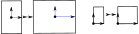
\includegraphics[width=\textwidth]{pics/linear/scale.pdf}
    \begin{align*}
        (1,0,0)&\rightarrow(x,0,0) & (0,1,0)&\rightarrow(0,y,0) & (0,0,1)&\rightarrow(0,0,z)
    \end{align*}
    \pause
    \begin{align*}
        S(x, y, z) &= \begin{pmatrix}
            x & 0 & 0 \\
            0 & y & 0 \\
            0 & 0 & z
        \end{pmatrix} \\
        S(x, y, z)^{-1} &= S(x^{-1}, y^{-1}, z^{-1}) \\
        \det S(x,y,z) &= xyz 
    \end{align*}
\end{frame}

\begin{frame}
    \frametitle{Rotace}

    Elementární rotace 
    \begin{align*}
        R_x(\alpha) &= \begin{pmatrix}
                1 & 0 & 0 \\
                0 & \cos \alpha & -\sin \alpha \\
                0 & \sin \alpha & \cos \alpha
            \end{pmatrix} &
        R_y(\alpha) &= \begin{pmatrix}
                \cos \alpha & 0 & \sin \alpha \\
                0 & 1 & 0 \\
                -\sin \alpha & 0 & \cos \alpha
            \end{pmatrix} \\
        R_z(\alpha) &= \begin{pmatrix}
                \cos \alpha & -\sin \alpha & 0 \\
                \sin \alpha & \cos \alpha & 0 \\
                0 & 0 & 1
            \end{pmatrix}
    \end{align*}

    \vfill

    Eulerovy úhly $\alpha, \beta, \gamma$
    \begin{equation*}
        R_x(\alpha)R_y(\beta)R_z(\gamma) \ne R_z(\gamma)R_y(\beta)R_x(\alpha)
    \end{equation*}
    \begin{itemize}
        \item[\color{red}:(] Nepraktické, neintuitivní, moc kombinací.
        \item[\color{red}:(] První otočení otáčí další osy $\rightarrow$ špatně se skládají.
    \end{itemize}
\end{frame}

\begin{frame}
    \frametitle{Lepší reprezentace rotací}

    Osa rotace $\NV{e} = (x,y,z)$ a úhel $\theta$
    \begin{align*}
        R((x,y,z), \theta) = \begin{pmatrix}
            x^2(1-c) + c & xy(1-c) - zs & xz(1-c) + ys \\
            yx(1-c) + zs & y^2(1-c) + c & yz(1-c) + xs \\
            zx(1-c) - ys & zy(1-c) + xs & z^2(1-c) + c \end{pmatrix} \\
        c = \cos\theta, s = \sin\theta
    \end{align*}
    \vfill
    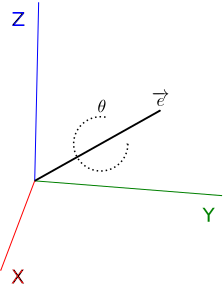
\includegraphics[height=.5\textheight]{pics/linear/axis-angle.pdf}
    \vfill
    Rodriguezův vzorec :
    \begin{equation*}
        \V{v}' = c\V{v} + s(\NV{e}\times\V{v}) + \NV{e}(\NV{e}\cdot\V{v})(1-c)
    \end{equation*}
\end{frame}

\begin{frame}
    \frametitle{Vlastnosti}
    Special Orthogonal Group $SO(3)$
    \begin{align*}
        \det R(\V{e}, \theta) &= 1 & {\color{blue}?} \\
        R(\V{e}, \theta)^{-1} &= R(\V{e}, \theta)^T = R(\V{e}, -\theta) \\
        R(\V{e}_1,\theta_1)\dotsm R(\V{e}_n,\theta_n) &= R(\dotso)
    \end{align*}
    \pause\vfill
    Orthogonal Group $O(3)$
    \begin{align*}
        \det F(\dotso) &= \pm1 & {\color{blue}?}
    \end{align*}
    \pause\vfill
    \begin{itemize}
        \item[\color{green}:)] Rotace + "Scale" = Zrcadlení
    \end{itemize}
    \begin{equation*}
        M(\NV{e}) = S(-1)R(\NV{e}, \pi)
    \end{equation*}
\end{frame}

\begin{frame}
    \frametitle{Posun}
    \begin{equation*}
        T(x,y,z) = \begin{pmatrix}
            1&0&0&x\\0&1&0&y\\0&0&1&z\\0&0&0&1
        \end{pmatrix}
    \end{equation*}
    \vfill
    \begin{equation*}
        T(\V{v})^{-1} = T(-\V{v})
    \end{equation*}
    \vfill
    \begin{itemize}
        \item Spolu s $SO(3)$ tvoří \textbf{Proper Rigid Transform}.
        \item Spolu s $O(3)$ tvoří \textbf{Rigid Transform}.
        \item Transformace pevného tìlesa.
    \end{itemize}
\end{frame}


\begin{frame}
    \frametitle{Skládání transformací}
    Asociativita
    \begin{equation*}
        F_1F_2\dotsb F_n\V{x} = (F_1F_2\dotsb F_n)\V{x}
    \end{equation*}
    \begin{itemize}
        \item Ve VS násobím jedinou maticí.
        \item Matice skládám při průchodu scénou.
    \end{itemize}
    \pause\vfill
    Inverzní transformace
    \begin{equation*}
        (F_1F_2\dotsb F_n)^{-1} = F_n^{-1}\dotsb F_2^{-1}F_1^{-1}
    \end{equation*}
    \begin{itemize}
        \item Při průchodu se dá složit i inverzní matice.
    \end{itemize}
\end{frame}

\begin{frame}
    \frametitle{Vyjádření maticí $4\times4$}
    \begin{itemize}
        \item Vektor $(x,y,z)^T \rightarrow (x,y,z,0)^T$
        \item Bod $(x,y,z)^T \rightarrow (x,y,z,1)^T$
        \item[\color{red}!!!] Tohle nejsou homogenní souřadnice!
    \end{itemize}
    \pause
    \begin{align*}
        \begin{pmatrix}
            F & \V{t} \\
            \V{0}^T & 1
        \end{pmatrix}\begin{pmatrix}\V{v}\\w\end{pmatrix}
        &= \begin{pmatrix}
            F\V{v} + {\color{blue}\V{t}w} \\
            \V{0}^T\V{v} + {\color{blue}1w}
        \end{pmatrix} \\
        \begin{pmatrix}
            3\times3 & 3\times1 \\
            1\times3 & 1\times1
        \end{pmatrix}\begin{pmatrix}3\times1\\1\times1\end{pmatrix}
        &= \begin{pmatrix}
            3\times3 \cdot 3\times1 + 3\times1 \cdot 1\times1 \\
            1\times3 \cdot 3\times1 + 1\times1 \cdot 1\times1
        \end{pmatrix}
    \end{align*}
    \pause\vfill
    Kombinace bodů a vektorů :
    \begin{align*}
        V + V &= V & 0+0 &= 0 \\
        P - P &= V & 1-1 &= 0 \\
        P \pm V &= P & 1\pm 0 &= 1 \\
        P + P &= \color{red}??? & 1+1 &= 2
    \end{align*}
\end{frame}



\begin{frame}
    \frametitle{Skládání}
    \begin{equation*}
        \begin{pmatrix}
            F_1 & \V{t}_1 \\
            \V{0}^T & 1
        \end{pmatrix}
        \begin{pmatrix}
            F_2 & \V{t}_2 \\
            \V{0}^T & 1
        \end{pmatrix}\V{p}
        = \begin{pmatrix}
            F_1F_2 + \V{t}_1\V{0}^T & F_1\V{t}_2 + \V{t}_11 \\
            \V{0}^TF_2 + 1\V{0}^T & \V{0}^T\V{t}_1 + 1\cdot1
        \end{pmatrix}\V{p}
    \end{equation*}
    \pause
    \begin{equation*}
        \begin{pmatrix}
            F_1F_2 & F_1\V{t}_2 + \V{t}_1 \\
            \V{0}^T & 1
        \end{pmatrix}
    \end{equation*}
    \pause\vfill
    Napřed $F$ a pak $T(\V{t})$ :
    \begin{equation*}
        \begin{pmatrix}
            F & \V{t} \\
            \V{0}^T & 1
        \end{pmatrix}
        =\begin{pmatrix}
            I & \V{t} \\
            \V{0}^T & 1
        \end{pmatrix}
        \begin{pmatrix}
            F & \V{0} \\
            \V{0}^T & 1
        \end{pmatrix}
    \end{equation*}
    \pause\vfill
    \begin{align*}
        (T(\V{t})F)^{-1} &= F^{-1}T(-\V{v}) \\
        \begin{pmatrix}
            F & \V{t} \\
            \V{0}^T & 1
        \end{pmatrix}^{-1}
        &= \begin{pmatrix}
            F^{-1} & -F^{-1}\V{t} \\
            \V{0}^T & 1
        \end{pmatrix}
    \end{align*}
\end{frame}

\begin{frame}
    \frametitle{Homogenní souřadnice}
    $\mathbf{RP}^N = \mathbb{R}^{N+1} \setminus \{\V{0}\}$ :
    \begin{itemize}
        \item N+1 souřadnic pro N-rozměrný prostor.
        \item[\color{red}!] Všechno jsou body.
        \item[\color{red}!] Ve 3D $(x, y, z, w)^T$ s aspoň jedním nenulovým prvkem.
        \item[\color{red}!] Každý bod má nekonečně mnoho reprezentací ($\V{p} \equiv k*\V{p}, k \in \mathbb{R} \setminus \{0\}$).
    \end{itemize}
    \pause\vfill
    $(x,y,z,0)$ jsou \textbf{ideální body} ležící v nekonečnu
    \begin{itemize}
        \item Leží ve směru vektoru $(x,y,z)$
        \item[\color{red}!!!] A zároveň i opačným směrem ($\V{p} \equiv -1\V{p}$)
        \item[\color{red}!!!] Nejsou to vektory, ty tu už nemáme.
    \end{itemize}
\end{frame}

\begin{frame}
    \frametitle{Projektivní prostor}
    \begin{itemize}
        \item Každý bod v $\mathbb{R}^3$ je přímka skrz počátek v $\mathbb{R}^4$.
        \item $k\V{p}$ je pohyb po té přímce.
        \item Počátkem procházejí všechny přímky, proto jsme ho odstranili.
        \item Perspektivní dělení počítá průsečík s rovinou $w = 1$.
    \end{itemize}
    \pause\vfill
    Projektivní rovina $\mathbf{RP}^2$
    \begin{itemize}
        \item Body $(x,y,z)$ bez $(0,0,0)$.
        \item Perspektivní dělení $(x,y,z) \rightarrow (x/z,y/z)$ promítá na rovinu $z=1$.
    \end{itemize}
\end{frame}

\setbeamercolor{background canvas}{bg=fitblue}
\begin{frame}
\frametitle{Projekce}
\begin{center}
\Huge {\color{white}Projekce}
\end{center}
\end{frame}
\setbeamercolor{background canvas}{bg=white}

\begin{frame}
\frametitle{Ortogonální projekce}
U ortogonální projekce je tvar pohledového tělesa kvádr.
Kvádr má 6 parametrů: l (left),r (right),b (bottom),t (top),n (near),f (far).
Kvádr je umístěn relativně ke středu souřadného systému.
\begin{figure}[htb]
	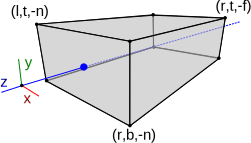
\includegraphics[height=4cm,keepaspectratio]{pics/projection/ortho}
	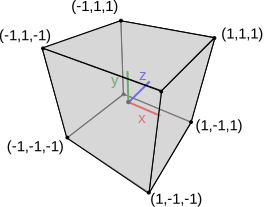
\includegraphics[height=4cm,keepaspectratio]{pics/projection/ndc}
\end{figure}
\end{frame}

\begin{frame}
\frametitle{Ortogonální projekce}
\begin{figure}[htb]
	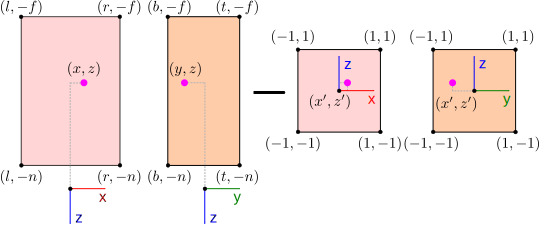
\includegraphics[height=4cm,keepaspectratio]{pics/projection/fromortho}
\end{figure}
\end{frame}

\begin{frame}
\frametitle{Ortogonální projekce}
\begin{multicols}{3}
{\tiny
\begin{eqnarray*}
	x &\in& [l,r] \\
	x-l &\in& [0,r-l] \\
	\frac{x-l}{r-l} &\in& [0,1] \\
	2 \frac{x-l}{r-l} &\in& [0,2] \\
	2 \frac{x-l}{r-l}-1 &\in& [-1,1]\\
	2 \frac{x-l}{r-l}- \frac{r-l}{r-l} &=& x'\\
	\frac{2}{r-l}x - \frac{r+l}{r-l} &=& x'
\end{eqnarray*}
}
\vfill
{\tiny
\begin{eqnarray*}
	y &\in& [b,t] \\
	y-b &\in& [0,t-b] \\
	\frac{y-b}{t-b} &\in& [0,1] \\
	2 \frac{y-b}{t-b} &\in& [0,2] \\
	2 \frac{y-b}{t-b}-1 &\in& [-1,1]\\
	2 \frac{y-b}{t-b}- \frac{t-b}{t-b} &=& y'\\
	\frac{2}{t-b}y - \frac{t+b}{t-b} &=& y'
\end{eqnarray*}
}
\vfill
{\tiny
\begin{eqnarray*}
	z &\in& [-n,-f] \\
	z+n &\in& [0,n-f] \\
	\frac{z+n}{n-f} &\in& [0,1] \\
	2 \frac{z+n}{n-f} &\in& [0,2] \\
	2 \frac{z+n}{n-f}-1 &\in& [-1,1]\\
	2 \frac{z+n}{n-f}- \frac{n-f}{n-f} &=& z'\\
	\frac{-2}{f-n}z + \frac{f+n}{f-n} &=& z'
\end{eqnarray*}
}
\end{multicols}

\end{frame}

\begin{frame}
\frametitle{Ortogonální projekce}
$$
\left[
\begin{array}{cccc} 
a_{1,1} & a_{1,2} & a_{1,3} & a_{1,4} \\
a_{2,1} & a_{2,2} & a_{2,3} & a_{2,4} \\
a_{3,1} & a_{3,2} & a_{3,3} & a_{3,4} \\
a_{4,1} & a_{4,2} & a_{4,3} & a_{4,4}
\end{array}
\right]
\cdot
\left[
\begin{array}{c}
x \\
y \\
z \\
1
\end{array}
\right]
=
\left[
\begin{array}{c} 
x' \\
y' \\
z' \\
1
\end{array}
\right]
=
\left[
\begin{array}{c} 
\frac{2}{r-l}x - \frac{r+l}{r-l}\\
\frac{2}{t-b}y - \frac{t+b}{t-b}\\
\frac{-2}{f-n}z + \frac{f+n}{f-n}\\
1
\end{array}
\right]
$$

$$
\left[
\begin{array}{cccc} 
\frac{2}{r-l} & 0             & 0              & -\frac{r+l}{r-l} \\
0             & \frac{2}{t-b} & 0              & -\frac{t+b}{t-b} \\
0             & 0             & \frac{-2}{f-n} & \frac{f+n}{f-n} \\
0             & 0             & 0              & 1
\end{array}
\right]
\cdot
\left[
\begin{array}{c}
x \\
y \\
z \\
1
\end{array}
\right]
=
\left[
\begin{array}{c} 
x' \\
y' \\
z' \\
1
\end{array}
\right]
$$
\end{frame}

\begin{frame}
\frametitle{Perspektivní projekce}
U perspektivní projekce je tvar pohledového tělesa komolý jehlan.
Stejně jako u Ortogonální projekce má 6 parametrů: l (left),r (right),b (bottom),t (top),n (near),f (far).
Jehlan je umístěn relativně ke středu systému.
\begin{figure}[htb]
	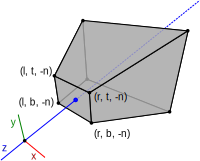
\includegraphics[height=4cm,keepaspectratio]{pics/projection/pers}
	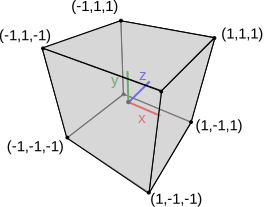
\includegraphics[height=4cm,keepaspectratio]{pics/projection/ndc}
\end{figure}
\end{frame}

\begin{frame}
\frametitle{Perspektivní projekce}
\begin{figure}[htb]
	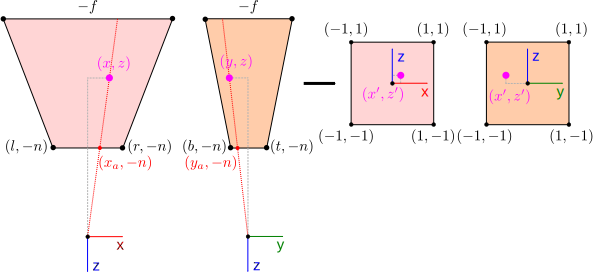
\includegraphics[height=5cm,keepaspectratio]{pics/projection/frompers}
\end{figure}
\end{frame}

\begin{frame}
\frametitle{Perspektivní projekce}
\begin{multicols}{2}
{\tiny
\begin{eqnarray*}
	\frac{x_a}{-n} &=& \frac{x}{z} \\
	x_a &=& \frac{-nx}{z} \\
	x_a &\in& [l,r] \\
	x_a-l &\in& [0,r-l] \\
	\frac{x_a-l}{r-l} &\in& [0,1] \\
	2\frac{x_a-l}{r-l}-1 &\in& [-1,1] \\
	\frac{2}{r-l}x_a-\frac{r+l}{r-l} &=& x'\\
	\frac{-2n}{r-l} \frac{x}{z} - \frac{r+l}{r-l} &=& x'
\end{eqnarray*}
\begin{equation}
\label{eq:persx}
\frac{-2n}{r-l} \frac{x}{z} - \frac{r+l}{r-l} = x'
\end{equation}
}
\vfill
{\tiny
\begin{eqnarray*}
	\frac{y_a}{-n} &=& \frac{y}{z} \\
	y_a &=& \frac{-ny}{z} \\
	y_a &\in& [b,t] \\
	y_a-b &\in& [0,t-b] \\
	\frac{y_a-b}{t-b} &\in& [0,1] \\
	2\frac{y_a-b}{t-b}-1 &\in& [-1,1] \\
	\frac{2}{t-b}y_a-\frac{t+b}{t-b} &=& y'\\
	\frac{-2n}{t-b} \frac{y}{z} - \frac{t+b}{t-b} &=& y'
\end{eqnarray*}
\begin{equation}
\label{eq:persy}
\frac{-2n}{t-b} \frac{y}{z} - \frac{t+b}{t-b} = y'
\end{equation}
}
\end{multicols}

\end{frame}

\begin{frame}
\frametitle{Perspektivní projekce, problém se z}
\begin{multicols}{2}
{\tiny
\begin{eqnarray*}
	z &\in& [-n,-f] \\
	z+n &\in& [0,n-f] \\
	\frac{z+n}{n-f} &\in& [0,1] \\
	2\frac{z+n}{n-f}-1 &\in& [-1,1] \\
	\frac{2}{n-f}z+\frac{n+f}{n-f} &=& z'
\end{eqnarray*}
\begin{equation}
\label{eq:linz}
\frac{2}{n-f}z+\frac{n+f}{n-f} = z'
\end{equation}
}
\vfill
{\tiny
\begin{eqnarray*}
	\frac{1}{z} &\in& [-\frac{1}{n},-\frac{1}{f}] \\
	\frac{1}{z}+\frac{1}{n} &\in& [0,\frac{f-n}{nf}] \\
	\frac{nf}{f-n}\frac{1}{z}+\frac{f}{f-n} &\in& [0,1] \\
	\frac{2nf}{f-n}\frac{1}{z}+\frac{2f}{f-n}-1 &\in& [-1,1] \\
\end{eqnarray*}
\begin{equation}
\label{eq:persz}
\frac{2nf}{f-n}\frac{1}{z}+\frac{f+n}{f-n} = z'
\end{equation}
}
\end{multicols}

\end{frame}

\begin{frame}
\frametitle{Perspektivní projekce}
{\tiny
\begin{equation}
\label{eq:swap}
\left[
\begin{array}{cccc} 
1 & 0 & 0 & 0 \\
0 & 1 & 0 & 0 \\
0 & 0 & 0 & 1 \\
0 & 0 & 1 & 0
\end{array}
\right]
\cdot
\left[
\begin{array}{c}
x \\
y \\
z \\
1
\end{array}
\right]
=
\left[
\begin{array}{c} 
x \\
y \\
1 \\
z
\end{array}
\right]
\end{equation}
}
\end{frame}

\begin{frame}
\frametitle{Perspektivní projekce}
{\tiny
\begin{equation}
\label{eq:persmat1}
\left[
\begin{array}{cccc} 
-\frac{2n}{r-l} & 0               & 0                & -\frac{r+l}{r-l} \\
0               & -\frac{2n}{t-b} & 0                & -\frac{t+b}{t-b} \\
0               & 0               & \frac{2nf}{f-n} & \frac{f+n}{f-n} \\
0               & 0               & 0                & 1
\end{array}
\right]
\cdot
\left[
\begin{array}{c}
x \\
y \\
1 \\
z
\end{array}
\right]
=
\left[
\begin{array}{c}
x'\cdot z \\
y'\cdot z \\
z'\cdot z \\
z
\end{array}
\right]
\end{equation}
}
\end{frame}

\begin{frame}
\frametitle{Perspektivní projekce}
Matice pro prohození $z$ a $w$ složky v homogenních souřadnicích:
{\tiny
\begin{equation}
\left[
\begin{array}{cccc} 
-\frac{2n}{r-l} & 0               & 0               & -\frac{r+l}{r-l} \\
0               & -\frac{2n}{t-b} & 0               & -\frac{t+b}{t-b} \\
0               & 0               & \frac{2nf}{f-n} & \frac{f+n}{f-n} \\
0               & 0               & 0               & 1
\end{array}
\right]
\cdot
\left[
\begin{array}{cccc} 
1 & 0 & 0 & 0 \\
0 & 1 & 0 & 0 \\
0 & 0 & 0 & 1 \\
0 & 0 & 1 & 0
\end{array}
\right]
=
\left[
\begin{array}{cccc} 
-\frac{2n}{r-l} & 0               & -\frac{r+l}{r-l} & 0 \\
0               & -\frac{2n}{t-b} & -\frac{t+b}{t-b} & 0 \\
0               & 0               & \frac{f+n}{f-n} & \frac{2nf}{f-n} \\
0               & 0               & 1                & 0
\end{array}
\right]
\end{equation}
}
\end{frame}

\begin{frame}
\frametitle{Perspektivní projekce}
{\tiny
\begin{equation}
\left[
\begin{array}{cccc} 
\frac{2n}{r-l} & 0               & \frac{r+l}{r-l} & 0 \\
0               & \frac{2n}{t-b} & \frac{t+b}{t-b} & 0 \\
0               & 0               & -\frac{f+n}{f-n} & -\frac{2nf}{f-n} \\
0               & 0               & -1                & 0
\end{array}
\right]
\cdot
\left[
\begin{array}{c}
x \\
y \\
z \\
1
\end{array}
\right]
=
\left[
\begin{array}{c}
-x'\cdot z \\
-y'\cdot z \\
-z'\cdot z \\
-z
\end{array}
\right]
\end{equation}
}
\end{frame}


\setbeamercolor{background canvas}{bg=fitblue}
\begin{frame}
\frametitle{Quaternions / Kvaterniony}
\begin{center}
\Huge {\color{white}Quaternions / Kvaterniony}
\end{center}
\end{frame}
\setbeamercolor{background canvas}{bg=white}


\begin{frame}\frametitle{Introduction / Úvod}\scriptsize
	\begin{itemize}
	\item Quaternion is extension of complex numbers into fourth dimension.
	\item Quaternion: $p=(a,b,c,d)$, $a$ is scalar/real part, $(b,c,d)$ is imaginary part.
	\item Quaternion: $(0,b,c,d)$ pure imaginary quaternion.
	\item Quaternion is constructed using Cayley-Dickson construction.
	\end{itemize}
	\begin{itemize}
	\item Kvaternion je rozšířením komplexních čísel do čtvrté dimenze.
	\item Kvaternion: $p=(a,b,c,d)$, $a$ je skalární část, $(b,c,d)$ je imaginární část.
	\item Kvaternion: $(0,b,c,d)$ se nazývá ryzí kvaternion.
	\item Kvaternion je sestrojen pomocí Cayley-Dickson konstrukce.
	\end{itemize}
\end{frame}

\begin{frame}\frametitle{Cayley-Dickson}\scriptsize
	\begin{itemize}
	\item Cayley-Dickson generalized construction of hypercomplex numbers.
	\item Construction produces algebras built on real numbers.
	\item Every algebra has $2\times$ higher dimension.
	\item With growing dimension, some properties are lost: commutativity, associativity, ...
	\item The construction begins at $\mathbb{R}$.
	\end{itemize}
	\begin{itemize}
	\item Cayley-Dickson zobecňuje postup konstrukce hyperkomplexních čísel.
	\item Konstrukce produkuje algebry nad reálnými čísly.
	\item Každá má $2\times$ vyšší dimenzi.
	\item S vyšší dimenzí ztrácejí vlastnosti: komutativnost násobení, asociativitu, ...
	\item Konstrukce začíná $\mathbb{R}$.
	\end{itemize}
\end{frame}

\begin{frame}\frametitle{Cayley-Dickson - complex numbers / komplexní čísla}\scriptsize
	\begin{itemize}
	\item A tuple of two real numbers $(a,b)$ can be viewed as complex number.
	\item For two complex numbers $p=(a,b),q=(c,d)$, these operation are defined:
	\end{itemize} 
	\begin{itemize}
	\item Dvojici reálných čísel $(a,b)$, lze uvažovat jako komplexní číslo.
	\item Pro dvojici komplexních čísel $p=(a,b),q=(c,d)$ jsou definovány operace:
	\end{itemize} 
\begin{eqnarray*}
p+q&=& (a,b)+(c,d)=(a+b,b+d)\\
k\cdot p &=& k\cdot (a,b)=(ka,kb),k \in \mathbb{R}\\
p\cdot q &=& (a,b) \cdot (c,d) = (ac-bd,ad+bc)\\
p^*&=&(a,b)^*=(a,-b)
\end{eqnarray*}
\end{frame}

\begin{frame}\frametitle{Couple of complex numbers / dvojice komplexních čísel}\scriptsize
	\begin{itemize}
	\item A tuple of two complex numbers $(p,q)$ can be viewed as couple of coule of real numbers.
	\item A couple of couple of real numbers $((a,b),(c,d))$ represents a quaternion.
	\item For two quaterions $p=(a,b),q=(c,d)$, the operations of multiplication and conjugation are defined differently:
	\end{itemize} 
	\begin{itemize}
	\item Dvojici komplexních čísel $(p,q)$ si můžeme představit jako dvojici dvojic reálných čísel.
	\item Dvojice dvojic reálných čísel $((a,b),(c,d))$ označujeme jako kvaternion.
	\item Pro dva kvaterniony $p=(a,b),q=(c,d)$ jsou operace násobení a konjugace definovány odlišně:
	\end{itemize} 
\begin{eqnarray*}
p\cdot q &=& (a,b) \cdot (c,d) = (ac-d^*b,da+bc^*)\\
p^*&=&(a,b)^*=(a^*,-b)
\end{eqnarray*}
\end{frame}

\begin{frame}\frametitle{Cayley-Dickson - generalization / zobecnění}\scriptsize
\begin{itemize}
  \item Two hypercomplex numbers $p=(a,b),q=(c,d)$ are formed from hypercomplex components (in lower dimension).
	\item Multiplication and conjugation are defined as follows:
\end{itemize} 
\begin{itemize}
	\item Dvě hyperkomplexní čísla $p=(a,b),q=(c,d)$ jsou složena z hyperkomplexních komponent, které jsou v nižší dimenzi.
	\item Násobení a konjugace jsou definovány následovně:
\end{itemize} 

\begin{eqnarray*}
p\cdot q &=& (a,b) \cdot (c,d) = (ac-d^*b,da+bc^*)\\
p^*&=&(a,b)^*=(a^*,-b)
\end{eqnarray*}

\begin{itemize}
 \item If $a$ is real number: $a^*=a, a \in \mathbb{R}.$
 \item Real numbers $\rightarrow$ complex numbers $\rightarrow$ quaternions $\rightarrow$ octonions, ...
 \item The dimension grows by factor of $2$.
\end{itemize} 
\begin{itemize}
 \item V případě, že konjugujeme reálné číslo: $a^*=a, a \in \mathbb{R}.$
 \item Postupnou konstrukcí z reálných čísel vznikají nejprve komplexní čísla, pak kvaterniony, oktoniony, ...
 \item Každý s dimenzí $2\times$ větší než předcházející.
\end{itemize} 
\end{frame}

\begin{frame}\frametitle{Notation / Značení}\scriptsize
\begin{itemize}
\item Symbol $i$ is used to mark imaginary component of complex numbers.
\item Components of quaternion $p=((a,b),(c,d))$ built using Cayley-Dickson construction are marked as follows:
\end{itemize}
\begin{itemize}
\item U komplexních čísel používáme symbol $i$ pro označení komplexní části.
\item U kvaternionů zkonstruovaných pomocí Cayley-Dickson konstrukce $p=((a,b),(c,d))$ označíme komponenty následovně:
\end{itemize}
\begin{eqnarray*}
p &=& ((a,b),(c,d))\\
p &=& ((a,bi),(c,di)j)\\
p &=& ((a,bi,(cj,dij))\\
p &=& a+bi+cj+dij
\end{eqnarray*}
\begin{itemize}
\item If $ij=k$ then we have hybercomplex number: $a+bi+cj+dk$.
\item There is scalar+vector notion of quaternion: $p=(s,\vec v)$.
\end{itemize}

\begin{itemize}
\item Pokud označíme součin $ij=k$ vznikne hyperkomplexní číslo: $a+bi+cj+dk$.
\item Další značení je pomocí skaláru a vektoru: $p=(s,\vec v)$.
\end{itemize}
\end{frame}

\begin{frame}\frametitle{Addition / Sčítání}\scriptsize
\begin{itemize}
\item Two quaternions $p=((a,b),(c,d)),q=((x,y),(z,w))$ can be added together as follows:
\item Kvaterniony $p=((a,b),(c,d)),q=((x,y),(z,w))$ se sčítají po složkách:
\end{itemize}
\begin{eqnarray*}
p+q &=& ((a,b),(c,d))+((x,y),(z,w))\\
p+q &=& ((a,b)+(x,y),(c,d)+(z,w))\\
p+q &=& ((a+x,b+y),(c+z,d+w))
\end{eqnarray*}
\begin{itemize}
\item Quaterion addition is commutative and associative.
\item Quaterion $((0,0),(0,0))$ represents identity for addition.
\end{itemize}
\begin{itemize}
\item Sčítání kvaternionů je komutativní a asociativní.
\item Kvaternion $((0,0),(0,0))$ představuje neutrální prvek ke sčítání.
\end{itemize}
\end{frame}

\begin{frame}\frametitle{Konjugace kvaternionu}\scriptsize
\begin{itemize}
\item Quaterion conjugation of quaterion $p=((a,b),(c,d))$:
\item Konjugace kvaternionu $p=((a,b),(c,d))$:
\end{itemize}
\begin{eqnarray*}
p^* &=& ((a,b),(c,d))^*\\
p^* &=& ((a,b)^*,-(c,d))\\
p^* &=& ((a^*,-b),(-c,-d))\\
p^* &=& ((a,-b),(-c,-d))
\end{eqnarray*}
\begin{itemize}
\item Vector notation: $p=(s,\vec v)$, $p^*=(s,-\vec v)$.
\item Conjugation of multiplication is: $(p \cdot q)^*= q^* \cdot p^*$.
\end{itemize}
\begin{itemize}
\item Při vektorovém zápisu $p=(s,\vec v)$, $p^*=(s,-\vec v)$.
\item Pro konjugaci součinu kvaternionů platí: $(p \cdot q)^*= q^* \cdot p^*$.
\end{itemize}
\end{frame}

\begin{frame}\frametitle{Multiplication / Násobení}\scriptsize
\begin{itemize}
\item Multiplication is not commutative: $p\cdot q \neq q \cdot p$.
\item Multiplication is associative: $p\cdot(q\cdot r)=(p\cdot q)\cdot r$.
\item Multiplication of quaternions acording Cayley-Dickson construction:
\end{itemize}
\begin{itemize}
\item Násobení kvaternionů není komutativní $p\cdot q \neq q \cdot p$.
\item Násobení kvaternionů je asociativní $p\cdot(q\cdot r)=(p\cdot q)\cdot r$.
\item Násobení kvaternionů podle Cayley-Dickson konstrukce:
\end{itemize}
{\tiny
\begin{eqnarray*}
p\cdot q &=& ((a,b),(c,d))\cdot((x,y),(z,w))\\
p\cdot q &=& ((a,b)\cdot(x,y)-(z,w)^*\cdot(c,d),(z,w)\cdot(a,b)+(c,d)\cdot(x,y)^*)\\
p\cdot q &=& ((a,b)\cdot(x,y)-(z^*,-w)\cdot(c,d),(z,w)\cdot(a,b)+(c,d)\cdot(x^*,-y))\\
p\cdot q &=& ((a,b)\cdot(x,y)-(z,-w)\cdot(c,d),(z,w)\cdot(a,b)+(c,d)\cdot(x,-y))\\
p\cdot q &=& ((ax-y^*b,ya+bx^*)-(zc+d^*w,dz-wc^*),(za-b^*w,bz+wa^*)+(cx+y^*d,-yc+dx^*))\\
p\cdot q &=& ((ax-yb,ya+bx)-(zc+dw,dz-wc),(za-bw,bz+wa)+(cx+yd,-yc+dx))\\
p\cdot q &=& ((ax-by-cz-dw,ay+bx+cw-dz),(az-bw+cx+dy,aw+bz-cy+dx))
\end{eqnarray*}
}
\end{frame}

\begin{frame}\frametitle{Multiplication / Násobení}\scriptsize

\begin{itemize}
\item Kvaterniony: $p=a+bi+cj+dk,q=x+yi+zj+wk$ can be multiplied together with following equality:
\item Kvaterniony ve tvaru: $p=a+bi+cj+dk,q=x+yi+zj+wk$ mohou být násobeny po složkách při dodržení rovnosti:
\end{itemize}

$$i^2=j^2=k^2=ijk=-1$$

\begin{itemize}
\item For the equality can be derived other rules:
\item Z rovnosti plynout další pravidla:
\end{itemize}

\begin{eqnarray*}
ijk &=& -1\\
iijk &=& -i\\
-jk &=& -i\\
jk &=& i
\end{eqnarray*}
\end{frame}

\begin{frame}\frametitle{Multiplication / Násobení}\scriptsize
\begin{itemize}
\item From the equality $i^2=j^2=k^2=ijk=-1$, the following table can be obtained by multiplication using $i,j,k$:
\item Z rovnosti $i^2=j^2=k^2=ijk=-1$ můžeme pomocí násobení $i,j,k$ postupně obdržet tabulku:
\end{itemize}
\begin{table}
\centering
\begin{tabular}{ |l||l|l|l|l| }
\hline
$\times$ & 1 & i & j & k \\
\hline
\hline
1 & 1 &  i &  j &  k \\
\hline
i & i & -1 &  k & -j \\
\hline
j & j & -k & -1 &  i \\
\hline
k & k &  j & -i & -1 \\
\hline
\end{tabular}
\end{table}
\end{frame}

\begin{frame}\frametitle{Násobení kvaternionů}\scriptsize
\begin{itemize}
\item Quaternions in scalar+vector from: $p=(s_1,\vec u),q=(s_2,\vec v)$ can be multiplied using scalar and vector multiplication:
\item Kvaterniony ve tvaru $p=(s_1,\vec u),q=(s_2,\vec v)$ lze vynásobit s pomocí skalárního a vektorového součinu:
\end{itemize}
\begin{eqnarray*}
p\cdot q &=& (s_1,\vec u),q=(s_2,\vec v)\\
p\cdot q &=& (s_1s_2-\vec u\cdot \vec v,\vec u \times \vec v + s_1\cdot \vec v + s_2 \cdot \vec u)
\end{eqnarray*}
\end{frame}

\begin{frame}\frametitle{Quaternion norm / Norma kvaternionů}\scriptsize
\begin{itemize}
  \item Norm of quaterion $q=((a,b),(c,d))$ is defined as  $\sqrt{q \cdot q^*}$:
  \item Norma kvaternionů $q=((a,b),(c,d))$ je definována jako odmocnina ze součinu kvaternionu $q$ a konjugovaného kvaternionu $q^*$:
\end{itemize}
\begin{eqnarray*}
||q|| &=& \sqrt{q \cdot q^*}\\
||q|| &=& \sqrt{((a,b),(c,d)) \cdot ((a,b),(c,d))^*}\\
||q|| &=& \sqrt{((a,b),(c,d)) \cdot ((a,-b),(-c,-d))}\\
||q|| &=& \sqrt{(a^2+b^2+c^2+d^2,0,(0,0))}\\
||q|| &=& (\sqrt{a^2+b^2+c^2+d^2},0,(0,0))\\
||q|| &=& \sqrt{a^2+b^2+c^2+d^2}
\end{eqnarray*}

\end{frame}

\begin{frame}\frametitle{Properties / Vlastnosti}\scriptsize
\begin{itemize}
\item Quaternions $p=(s_1,\vec u),q=(s_2,\vec v)$ are parallel if vectors $\vec u,\vec v$ are parallel.
\item Quaternions $p,q$ are perpendicular if vector $\vec u,\vec v$ are perpendicular.
\item Multiplication $p \cdot q$ of two pure vector quaternions $p=(0,\vec u),q=(0,\vec v)$ is pure vector quaternion $(0,\vec u \times \vec v)$ only if they are perpendicular.
\item Quaternion $p=(0,(0,0,0))$ is identity for addition.
\item Quaternoin $e=(1,(0,0,0))$ is identity for multiplication. For any $p$: $e\cdot p=p \cdot e = p$.
\item Inverse quaterion of $p$ for multiplication is quaterbuib $p^{-1}$, for which: $p\cdot p^{-1}=p^{-1}\cdot p=e$, $p\cdot p^*=||p||^2$, $p\cdot \frac{p^{*}}{||p||^2}=e,p^{-1}=\frac{p^*}{||p||^2}$.
\end{itemize}

\begin{itemize}
\item
Kvaterniony $p=(s_1,\vec u),q=(s_2,\vec v)$ jsou rovnoběžné v případě, že vektory $\vec u,\vec v$ jsou na sebe rovnoběžné.
\item
Kvaterniony $p,q$ jsou na sebe kolmé v případě, že vektory $\vec u,\vec v$ jsou na sebe kolmé.
\item
Součin $p \cdot q$ dvou ryzích kvaternionů $p=(0,\vec u),q=(0,\vec v)$ je ryzí kvaternion $(0,\vec u \times \vec v)$ jenom v případě, že jsou vektory $\vec u,\vec v$ na sebe kolmé.
\item
Kvaternion $p=(0,(0,0,0))$ je nulový kvaternion.
\item
Neutrální prvek vůči násobení je kvaternion $e=(1,(0,0,0))$.
Pro jakýkoliv kvaternion $p$ platí: $e\cdot p=p \cdot e = p$.
\item
Inverzní kvaternion ke kvaternionu $p$ vůči operaci násobení, je takový kvaternion $p^{-1}$, pro který platí: $p\cdot p^{-1}=p^{-1}\cdot p=e$.
Součin kvaternionu a jeho konjugace: $p\cdot p^*=||p||^2$.
Odtud $p\cdot \frac{p^{*}}{||p||^2}=e,p^{-1}=\frac{p^*}{||p||^2}$.
\end{itemize}
\end{frame}

\begin{frame}\frametitle{Rotace - Eulerovy úhly}\scriptsize
\begin{itemize}
\item Rotation in 3D space can be represented using three angles -- Euler angles.
\item Euler angles $\alpha,\beta,\gamma$ are used for three perpendicular exes.
\item Euler angles are closelly related to gimbal.
\item Gimbal lock -- loss of degree of freedom.
\item Quaternions do not suffer from gimbal lock.
\end{itemize}
\begin{itemize}
\item Rotace v 3D může být reprezentována pomocí tří úhlů - Eulerovy úhly.
\item Eulerovy úhly $\alpha,\beta,\gamma$ jsou použity pro tři na sebe kolmé osy.
\item Eulerovy úhly jsou blízké Kardanově závěsu.
\item Kardanův závěs v určité pozici ztrácí stupeň volnosti "Gimbal lock".
\item Kvaterniony tímto jevem netrpí.
\end{itemize}
\end{frame}

\begin{frame}\frametitle{Rotation / Rotace}\scriptsize
\begin{itemize}
\item Quaternion represents rotation as rotation around certaion exis using some angle.
\item Only unit quaternions are used for rotation: $||p||=1$.
\item Any unit quaternion can be written as: $(cos(\alpha),sin(\alpha)\cdot \vec v)$.
\item The angle is in range: $\alpha \in [0,\pi]$ and the vector is unit vector: $|\vec v|=1$.
\item If the angle is: $\alpha=0,\pi$, quaternion is: $((\pm 1,0),(0,0))$ -- identity.
\end{itemize}

\begin{itemize}
\item Kvaternion reprezentuje rotaci jako rotaci kolem určité osy o určitý úhel.
\item Pro rotaci pomocí kvaternionů se používají jednotkové kvaterniony $||p||=1$.
\item Jakýkoliv jednotkový kvaternion může být zapsán jako $(cos(\alpha),sin(\alpha)\cdot \vec v)$.
\item Úhel nabývá hodnot $\alpha \in [0,\pi]$ a vektor $|\vec v|=1$ je jednotkový.
\item Vektor $\vec v$ reprezentuje osu otáčení a úhel $\alpha$ reprezentuje úhel natočení.
\item Pro úhel $\alpha=0,\pi$ je kvaternion ve formě $((\pm 1,0),(0,0))$, což je neutrální prvek.
\end{itemize}
\end{frame}

\begin{frame}\frametitle{Rotation / Rotace}\scriptsize
\begin{itemize}
\item A point $r=(r_1,r_2,r_3)$, has to be converted to pure vector quaternion $p=((0,r_1),(r_2,r_3))$, if we want to rotate it.
\item Axis of rotation represented as unit vector $\vec v$, and angle $\alpha$ has to be converted to unit quaternion: $q=(cos(\frac{\alpha}{2}),sin(\frac{\alpha}{2})\cdot\vec v)$.
\item The rotation of point $r$ around axis $v$ using angle $\alpha$:
$$q\cdot p \cdot q^*=p'$$
\item $p'$ is rotated point.
\end{itemize}

\begin{itemize}
\item Bod $r=(r_1,r_2,r_3)$, který chceme rotovat převedeme na ryzí kvaternion: $p=((0,r_1),(r_2,r_3))$.
\item Osu, reprezentovanou pomocí jednotkového vektoru $\vec v$, a úhel $\alpha$, převedeme na jednotkový kvaternion: $q=(cos(\frac{\alpha}{2}),sin(\frac{\alpha}{2})\cdot\vec v)$.
\item Rotace bodu $r$ kolem osy $v$ o úhel $\alpha$:
$$q\cdot p \cdot q^*=p'$$
\item $p'$ představuje rotovaný bod.
\end{itemize}
\end{frame}

\begin{frame}\frametitle{Composition of rotations / Skládání rotací}\scriptsize
\begin{itemize}
\item Quaterion: $p=((0,r_1),(r_2,r_3))$ represents bod that we want to rotate.
\item Unit quaternions: $q,t$ represents two rotations.
\item Application of both rotations:
\end{itemize}

\begin{itemize}
\item Kvaternion: $p=((0,r_1),(r_2,r_3))$ reprezentuje bod, který chceme rotovat.
\item Jednotkové kvaterniony: $q,t$ reprezentují dvě rotace.
\item Aplikování rotací:
\end{itemize}

\begin{eqnarray*}
p' &=& t\cdot (q\cdot p \cdot q^*)\cdot t^*\\
p' &=& t\cdot q\cdot p \cdot q^*\cdot t^*\\
p' &=& (t\cdot q)\cdot p \cdot (q^*\cdot t^*)\\
p' &=& (t\cdot q)\cdot p \cdot (t \cdot q)^*\\
p' &=& s \cdot p \cdot s^*
\end{eqnarray*}

\begin{itemize}
\item Composition of $q,t$ forms new quaterion $s=q\cdot t$ that represents both rotations.
\item Složení rotací $q,t$ vznikne kvaternion $s=q\cdot t$, který reprezentuje obě rotace.
\end{itemize}
\end{frame}

\begin{frame}\frametitle{Conversion to matrices / Převod na rotační matici}\scriptsize
\begin{itemize}
\item Conversion of unit quaterion $(\cos(\frac{\alpha}{2}),\sin(\frac{\alpha}{2})\vec v)$ to rotation matrix:
\item Převod jednotkového kvaternionu $(\cos(\frac{\alpha}{2}),\sin(\frac{\alpha}{2})\vec v)$ na rotační matici:
\end{itemize}
{\tiny
$$
\left[
\begin{array}{ccc} 
\cos(\alpha)+v_x^2(1-\cos(\alpha))     & v_xv_y(1-\cos(\alpha))-v_z\sin(\alpha) & v_xv_z(1-\cos(\alpha))+v_y\sin(\alpha) \\
v_yv_x(1-\cos(\alpha))+v_z\sin(\alpha) & \cos(\alpha)+v_y^2(1-\cos(\alpha))       & v_yv_z(1-\cos(\alpha))-v_x\sin(\alpha) \\
v_zv_x(1-\cos(\alpha))-v_y\sin(\alpha) & v_zv_y(1-\cos(\alpha))+v_x\sin(\alpha) & \cos(\alpha)+v_z^2(1-\cos(\alpha)) \\
\end{array}
\right]
$$
}
\end{frame}


\setbeamercolor{background canvas}{bg=fitblue}
\begin{frame}
\frametitle{Duální kvaterniony}
\begin{center}
\Huge {\color{white} Duální kvaterniony}
\end{center}
\end{frame}
\setbeamercolor{background canvas}{bg=white}


\begin{frame}
\frametitle{Úvod}
	\begin{itemize}
	\item Matice lze použí pro mnoho druhů transformací: rotace, posuny, měřítko, projekci, ...
  \item Kvaternion lze použí pro rotace, posun je potřeba udělat separátně
  \item Eulerovy úhly lze použí pro rotace, posun je potřeba udělat separátně
  \item Úhel+osa lze použít pro rotace, posun je potřeba udělat separátně
  \item Duální kvaternion: umožňují rotace a posun
  \item Vhodné pro pohyb rigidních těles: posuny+rotace
  \item Jednotná reprezentace
  \item Kombinuje koncept kvaternionů a duálních čísel
	\end{itemize}
\end{frame}

\begin{frame}
\frametitle{Duální čísla}
	\begin{itemize}
	\item Podobné komplexním číslům.
  \item Komplexní číslo: $c = r+b \cdot i$, $r$ reálná část, $b$ imaginární část, $i^2 = -1$.
  \item Duální číslo: $z = r + d \cdot \epsilon$, $r$ reálná část, $d$ duální část, $\epsilon^2 = 0, \epsilon \neq 0$
  \item $\epsilon$ je duální operátor.
  \item Sčítání: $(r_a + d_a \cdot \epsilon) + (r_b + d_b \cdot \epsilon) = (r_a + r_b) + (d_a + d_b) \cdot \epsilon$
  \item Násobení: $(r_a + d_a \cdot \epsilon) \cdot (r_b + d_b \cdot \epsilon) = r_a \cdot r_b + (r_a \cdot d_b + d_a \cdot r_b) \cdot \epsilon $
  \item Dělení: podobně jako komplexní čísla - pomocí sdružených čísel $(r + d \cdot \epsilon)^* = (r - d \cdot \epsilon)$
	\end{itemize}
\end{frame}

\begin{frame}
\frametitle{Duální kvaterniony}
	\begin{itemize}
  \item Duální kvaterniony: dva kvaterniony, jeden reálný a druhý duální.
  \item $\mathbf{q} = \mathbf{q}_r + \mathbf{q}_d \cdot \epsilon$
  \item Násobení skalárem: $s \cdot \mathbf{q} = s \cdot \mathbf{q}_r + s \cdot \mathbf{q}_d \cdot \epsilon$
  \item Sčítání: $\mathbf{q}_1 + \mathbf{q}_2  = (\mathbf{q}_{r1}+\mathbf{q}_{r2}) + (\mathbf{q}_{d1} + \mathbf{q}_{d2}) \cdot \epsilon$
  \item Násobení: $\mathbf{q}_1 \cdot \mathbf{q}_2  = (\mathbf{q}_{r1} \cdot \mathbf{q}_{r2}) + (\mathbf{q}_{r1} \cdot \mathbf{q}_{d2} + \mathbf{q}_{d1} \cdot \mathbf{q}_{r2} ) \cdot \epsilon$
  \item Konjugace: $\mathbf{q^*} = \mathbf{q}_{r}^* + \mathbf{q}_{d}^* \cdot \epsilon$
  \item Velikost: $\left\lVert \mathbf{q} \right\rVert = \mathbf{q} \cdot \mathbf{q}^*$
  \item Podmínky: $\left\lVert \mathbf{q} \right\rVert = 1$, $\mathbf{q}_r^* \cdot \mathbf{q}_d + \mathbf{q}_d^* \cdot \mathbf{q}_r = 0$
  \item Pokud jsou podmínky splněny, duální kvaterniony reprezentují libovolnou rotaci a posun.
	\end{itemize}
\end{frame}

\begin{frame}
\frametitle{Sestavení duálního kvaternion}
	\begin{itemize}
  \item Reálný kvaternion reprezentuje rotaci: $\mathbf{q}_r = \mathbf{r}$, $\mathbf{r}$ je kvaternion reprezentující rotaci.
  \item Duální kvaternion reprezentuje polovinu rotace a posunu: $\mathbf{q}_d = \frac{1}{2} \cdot \mathbf{r} \cdot \mathbf{t}$.
  \item $\mathbf{t}$ je kvaternion $\mathbf{t} = (0,\mathbf{t}_x,\mathbf{t}_y,\mathbf{t}_z)$.
  \item Čistá rotace: $\mathbf{q}_r = \left(cos\left(\frac{\phi}{2}\right),\mathbf{n}_x \cdot sin\left(\frac{\phi}{2}\right),\mathbf{n}_y \cdot sin\left(\frac{\phi}{2}\right),\mathbf{n}_z \cdot sin\left(\frac{\phi}{2}\right),0,0,0,0\right)$
  \item Čistý posun: $\mathbf{q}_t = \left(1,0,0,0,0,\frac{\mathbf{t}_x}{2},\frac{\mathbf{t}_y}{2},\frac{\mathbf{t}_z}{2}\right)$
  \item Rotace pak transformace: $\mathbf{q} = \mathbf{q}_t \times \mathbf{q}_r$
  \item Transformování bodu: $\mathbf{p}' = \mathbf{q} \cdot \mathbf{p} \cdot \mathbf{q}^*$
	\end{itemize}
\end{frame}

\begin{frame}
\frametitle{Vlastnosti}
	\begin{itemize}
  \item Kombinování matic 4x4: 64 násobení, 48 sčítání
  \item Kombinování matic 4x3: 48 násobání, 32 sčítání
  \item Kombinování duálních kvaternionů: 42 násobení, 38 sčítání
  \item Je nutné zachovat jednotkové velikost a pořadí (stejné jako u matic)
  \item Je možné interpolovat (stejně jako kvaterniony)
  \item Nejsou singularity (gimbal lock)
  \item Jednotná reprezentace
  \item Nejkratší cesta interpolace
  \item Další čtení: \textbf{Ben Kenwright: A Beginners Guide to Dual-Quaternions}
	\end{itemize}
\end{frame}


\begin{frame}
  \frametitle{References}
  \begin{itemize}
    \item \url{http://www.opengl.org/sdk/docs/}
    \item \url{http://www.opengl.org/documentation/glsl/}
    \item \url{http://www.opengl.org/registry/}
  \end{itemize}
\end{frame}



\bluepage{Thank you for your attention! \vspace{10 mm} Questions?}

\end{document}
